% !TeX root = ./main.tex
\documentclass[11pt, a4paper, USenglish]{article} % change ``USenglish'' to ``norsk'' if applicable.

\setlength{\marginparwidth}{2cm}
\usepackage{kyblab} % Contains all included packages. See kyblab.sty.
\addbibresource{bibliography.bib} % Makes the bibliography file available to biblatex.

\begin{document}

% Titlepage
\title{TDT4195 - Visual Computing Fundamentals - Assignment 3}
\author{Group 119\\Martin Eek Gerhardsen}
\date{October 4th, 2019}
\begin{titlepage}
    \maketitle
    \begin{figure}
    \centering
    
\includegraphics[width=0.5\textwidth]{figures/itk_ntnu}\\
    Department of Engineering Cybernetics
    \end{figure}
    \thispagestyle{empty}
\end{titlepage}

% TOC
\newpage
\tableofcontents
\thispagestyle{empty} 

% Main content
\newpage
\setcounter{page}{1}
\section{Spatial Filtering}

\subsection{Task 1: Theory}
\subsubsection*{a)}
Sampling is the process of converting a continuos-time signal to a discrete-time signal, usually by measuring the continuos-time signal at specific points in time and extending this measurement over a set time step. 

\subsubsection*{b)}
Quantization is the process of constraining a signal from a larger to a smaller set of values, like mapping colours to the standard RGB range of 256 integer values. 

\subsubsection*{c)}
A high contrast image histogram would look similar to a dirac delta function, with most values grouped together around the same intensity.

\subsubsection*{d)}
\begin{table}[]
    \label{tab:initial_image}
    f = \begin{tabular}{|l|l|l|l|l|}
        \hline
        5 & 0 & 2 & 3 & 4 \\ \hline
        3 & 2 & 0 & 5 & 6 \\ \hline
        4 & 6 & 1 & 1 & 4 \\ \hline
    \end{tabular}
\end{table}
\begin{align*}
    n_{\text{pixel}} &= 3 * 5 = 15 \\
    L = 7
    i_0 &= 2 \\ 
    i_1 &= 2 \\
    i_2 &= 2 \\
    i_3 &= 2 \\
    i_4 &= 3 \\
    i_5 &= 2 \\
    i_6 &= 2 \\
    i_7 &= 0
\end{align*}
Then using \cref{eq:equalizer} on \cref{tab:initial_image} gives \cref{tab:equalized_image}. 

\begin{align*}
    \begin{bmatrix}
        n   & 0             & 1             & 2             & 3             & 4             & 5             & 6             & 7 \\ \hline
        f_n &\frac{2}{15} &\frac{2}{15} &\frac{2}{15} &\frac{2}{15} &\frac{3}{15} &\frac{2}{15} &\frac{2}{15} &\frac{0}{15} \\
        F_n &\frac{2}{15} &\frac{4}{15} &\frac{6}{15} &\frac{8}{15} &\frac{11}{15} &\frac{13}{15} &\frac{15}{15} &\frac{15}{15} \\
        E_q & 0 & 1 & 2 & 3 & 4 & 5 & 6 & 6
    \end{bmatrix}
\end{align*}

\begin{equation}
    \label{eq:equalizer}
    g_{i,j} = floor((L - 1) * \sum_{n = 0}^{f_{i,j}} \frac{i_n}{n_{\text{pixel}}}) = floor((L - 1) * F_n)
\end{equation}

\begin{table}[]
    \label{tab:equalized_image}
    \begin{tabular}{|l|l|l|l|l|}
        \hline
        6 & 0 & 2 & 3 & 4 \\ \hline
        3 & 2 & 0 & 5 & 6 \\ \hline
        4 & 6 & 1 & 1 & 4 \\ \hline
    \end{tabular}
\end{table}

\subsubsection*{e)}
The log transform will increase the output intensity for low input intensities, and flatten for high input intensities. This will make it easier to see the lower ranges of the input intensities. If we then apply this transform to 


\newpage
\subsection{Task 2: Programming}
\subsubsection*{a)}
See the result from \cref{fig:greyscale}. 
\begin{figure}[]
    \centering
    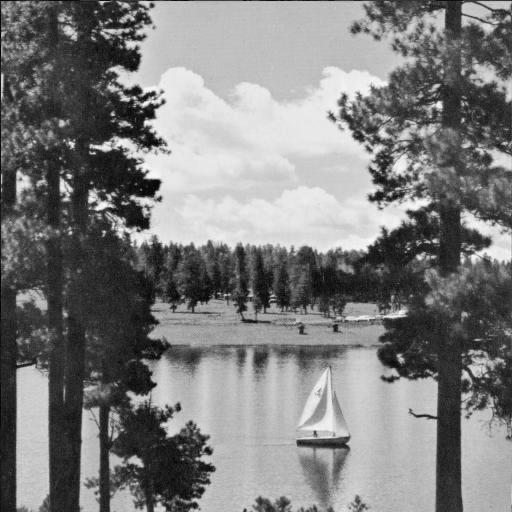
\includegraphics[width=1.00\textwidth]{figures/image_processed/lake_greyscale.jpg}
    \caption{The grey scale version of the lake image}
    \label{fig:greyscale}
\end{figure}

\subsubsection*{b)}
Se the result from \cref{fig:inverse}. 
\begin{figure}[]
    \centering
    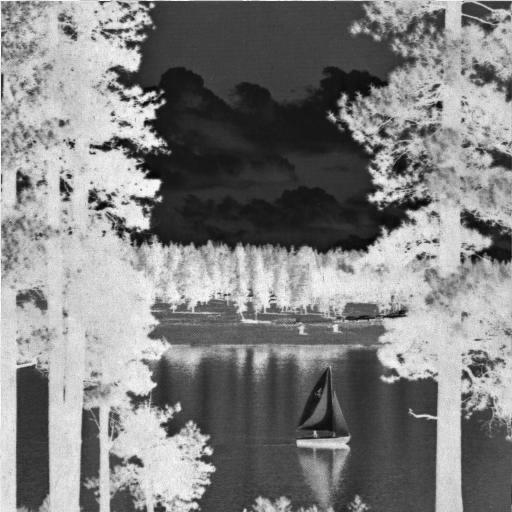
\includegraphics[width=1.00\textwidth]{figures/image_processed/lake_inverse.jpg}
    \caption{The inverse of the grey scale version of the lake image}
    \label{fig:inverse}
\end{figure}

\subsubsection*{c)}
See the results from \cref{fig:convolution_h_a} and \cref{fig:convolution_h_b}.

\begin{figure}[]
    \centering
    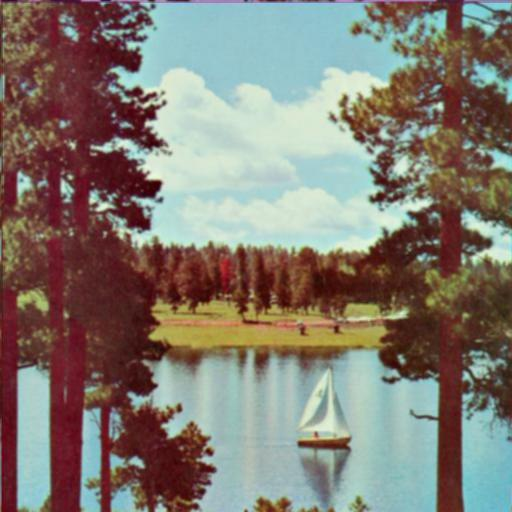
\includegraphics[width=1.00\textwidth]{figures/image_processed/convolved_im_h_a.jpg}
    \caption{Convolution of the lake image with the kernel $h_a$.}
    \label{fig:convolution_h_a}
\end{figure}

\begin{figure}[]
    \centering
    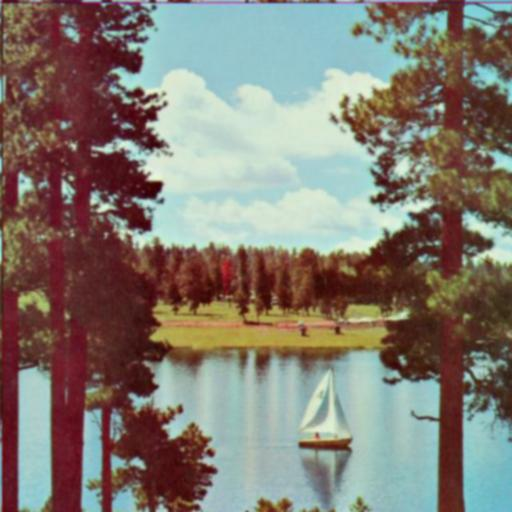
\includegraphics[width=1.00\textwidth]{figures/image_processed/convolved_im_h_b.jpg}
    \caption{Convolution of the lake image with the kernel $h_b$.}
    \label{fig:convolution_h_b}
\end{figure}

\section{Filtering in the Frequency Domain}
\subsection{Task 3: Theory}
\subsubsection*{a)}
From the convolution theorem, we can see that the Fourier transform of a convolution of two signals is multiplication of the Fourier transforms of those individual signals. So a stepwise description would be: 
\begin{itemize}
    \item Find the Fourier transform of the individual signals (i.e. using FFT)
    \item Pointwise multiply the transformed signals
    \item Use inverse Fourier transform to find the convolution of the original signals
\end{itemize}

\subsubsection*{b)}
Low- and high-pass filters tell us which frequencies should be kept, low-pass allows low frequencies to pass, and high-pass allows high frequencies to pass. 

This means that low-pass filters should be close to the filter gain (i.e. 1) frequencies closer to the origin than the cut-off frequency (low frequencies), and should be close to zero for higher frequencies than the cut-off frequency. Depending on how we want the filter to behave, the filter can either be similar to a cylinder or a cone, where cylinder gives a much \textit{harsher} cut-off frequency (no frequencies after cut-off) and cone gives a \textit{smoother} cut-off frequency (allowing, but suppressing some frequencies after cut-off). 

The high-pass filter is simply the $K - LPF$, where $K$ is the filter gain (i.e. 1 again) and $LPF$ is the low-pass filter. This implies that the high-pass filter follows the same pattern as the low-pass, but where the low-pass filter includes frequencies, the high-pass filter removes them, and vice versa where the high-pass includes the frequencies. 

\subsubsection*{c)}
As the images are shifted, we find the low frequencies in the centre and high around the image. Also using the white parts of the images as high amplitude, and black as low amplitude. 

a)
This is primarily a high-pass filter, as the lower frequencies are suppressed. This filter is primarily a high-pass filter along the y-axis (so high frequencies are only allowed given that they are along the y-axis), rather than both x and y. 

b)
This is a high-pass filter, the lower frequencies in the centre are largely suppressed, and the higher frequencies are multiplied with values closer to 1. Though, as the values closest to the x- and y-axes are slightly darker than the diagonals for high frequencies, the filter prefers the signal to have both high frequencies in x and y at the same time. 

c)
This is a low-pass filter, the lower frequencies in the centre are largely included, while the higher frequencies are suppressed.

\newpage
\subsection{Task 4: Programming}
\subsubsection*{a)}
The high-pass filtered image, with the amplitude of the Fourier transforms, can be seen from \cref{fig:camera_high_pass}, and similarly for the low-pass filtered image from \cref{fig:camera_low_pass}. 

\begin{figure}[]
    \centering
    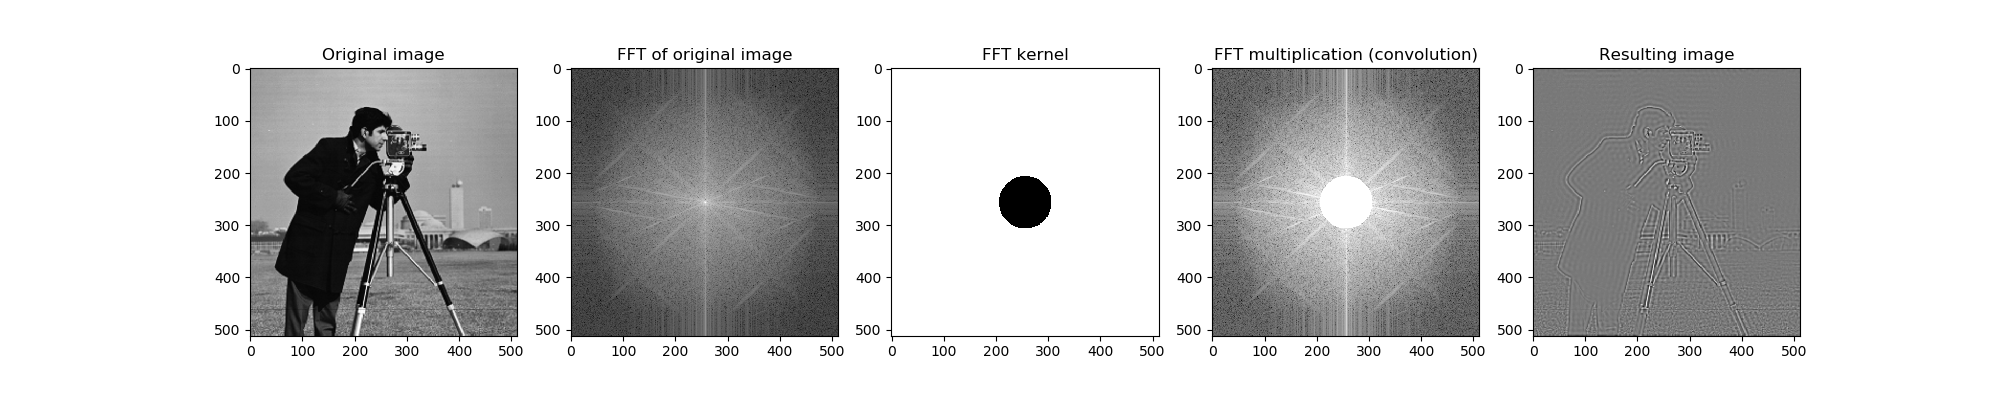
\includegraphics[width=1.00\textwidth]{figures/image_processed/camera_high_pass_subplots.png}
    \caption{High-pass filtered camera man}
    \label{fig:camera_high_pass}
\end{figure}

\begin{figure}[]
    \centering
    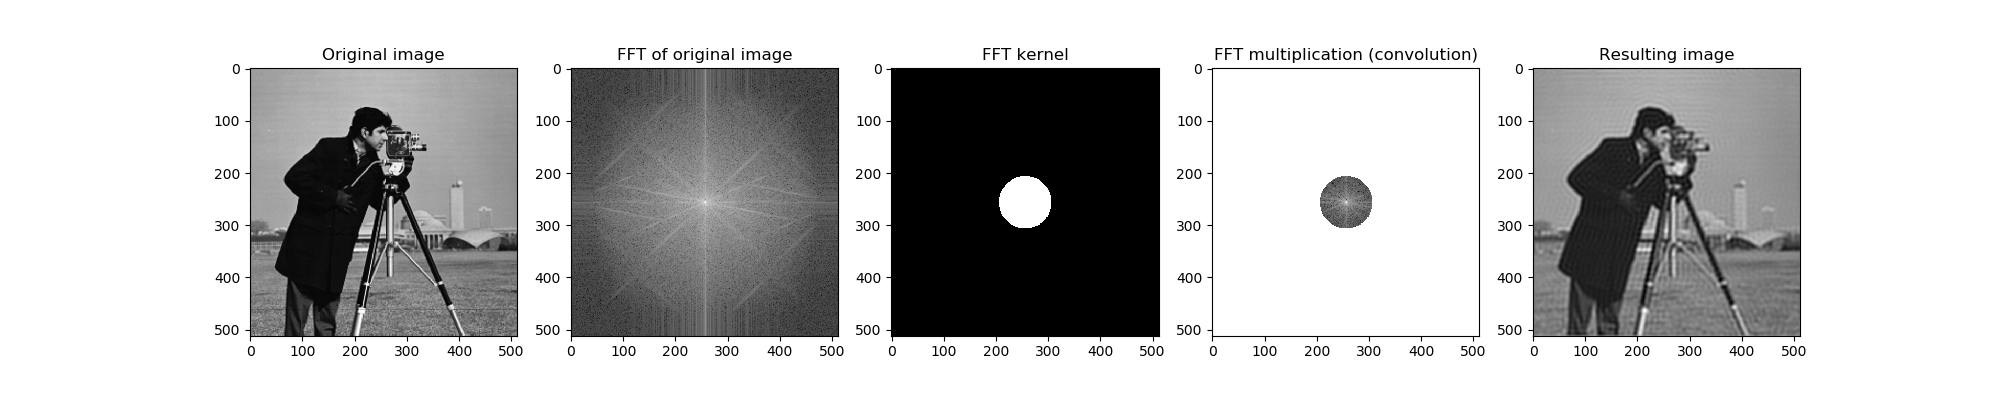
\includegraphics[width=1.00\textwidth]{figures/image_processed/camera_low_pass_subplots.png}
    \caption{Low-pass filtered camera man}
    \label{fig:camera_low_pass}
\end{figure}

\subsubsection*{b)}
The image convolution process for the gaussian kernel can be seen from \cref{fig:camera_gaussian}, and the image convolution process for the horizontal sobel filter can be seen from \cref{fig:camera_sobelx}

\begin{figure}[]
    \centering
    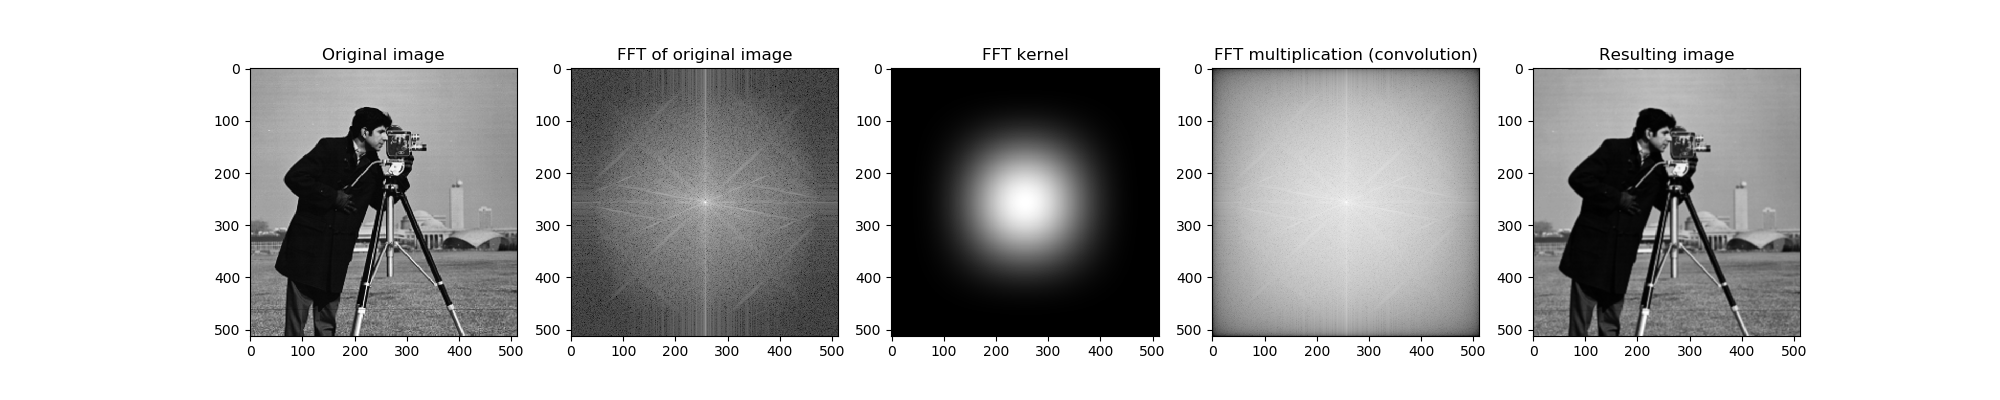
\includegraphics[width=1.00\textwidth]{figures/image_processed/camera_gaussian_subplots.png}
    \caption{Gaussian filtered camera man}
    \label{fig:camera_gaussian}
\end{figure}

\begin{figure}[]
    \centering
    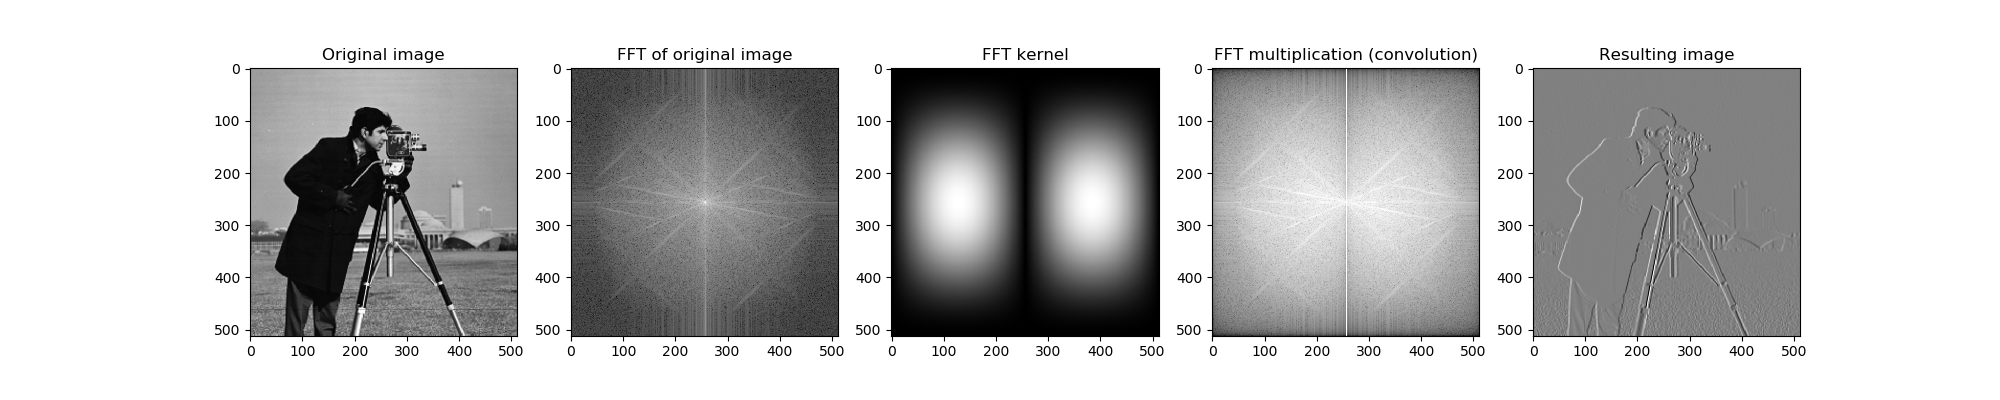
\includegraphics[width=1.00\textwidth]{figures/image_processed/camera_sobelx_subplots.png}
    \caption{Horizontal sobel filtered camera man}
    \label{fig:camera_sobelx}
\end{figure}

\subsubsection*{c)}
The image convolution process for the mystery-filtering can be seen from \cref{fig:clown_filtered}. It is pretty simple to see that this filter removes certain filter-bands, which implies that this is a combination of a four notch filters, or inverse bandpass filters. This then \textit{removes} certain bands of frequencies along the x-axis and y-axis. 

From the Fourier transform of the image, we can see that certain frequencies are very prevalent, and this filter removes those specific points. These were the primary causes for the picture being so wave-y before applying the filter. 

To conclude, I'd call this filter a notch filter (or more accurately a combination of four notch filters). 

\begin{figure}[]
    \centering
    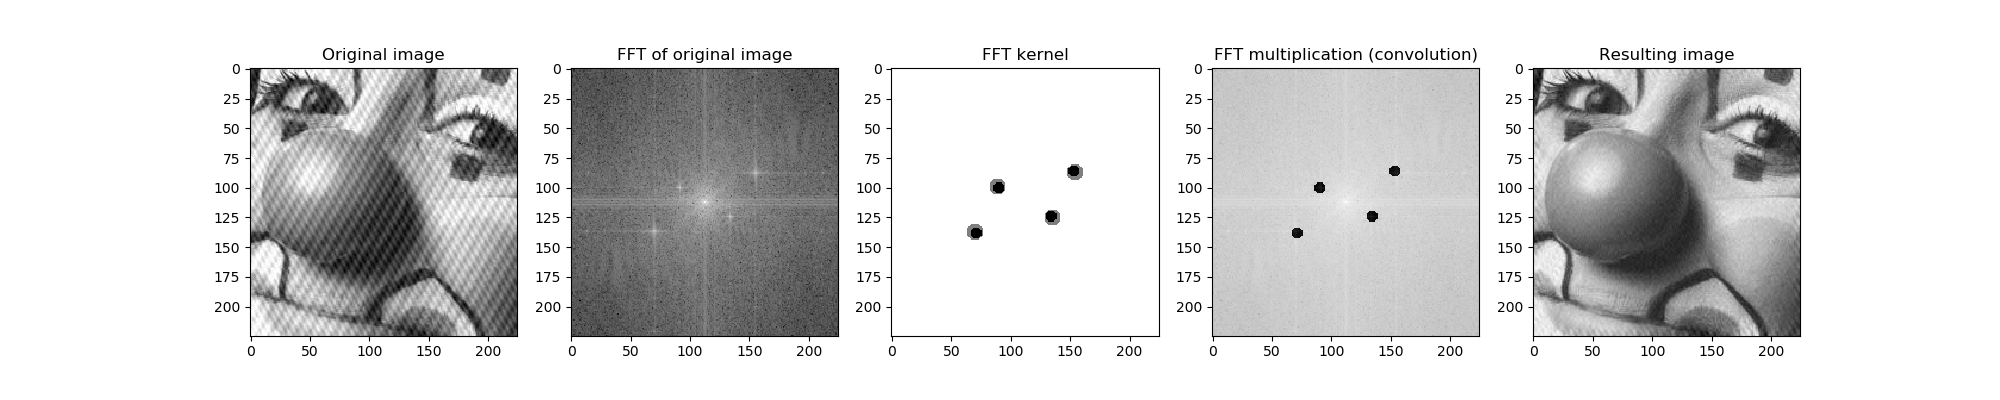
\includegraphics[width=1.00\textwidth]{figures/image_processed/clown_filtered_subplots.png}
    \caption{Mystery-filtered clown (notch filter)}
    \label{fig:clown_filtered}
\end{figure}

\subsubsection*{d)}
See the sharpened image from \cref{fig:moon_sharpened}.

\begin{figure}[]
    \centering
    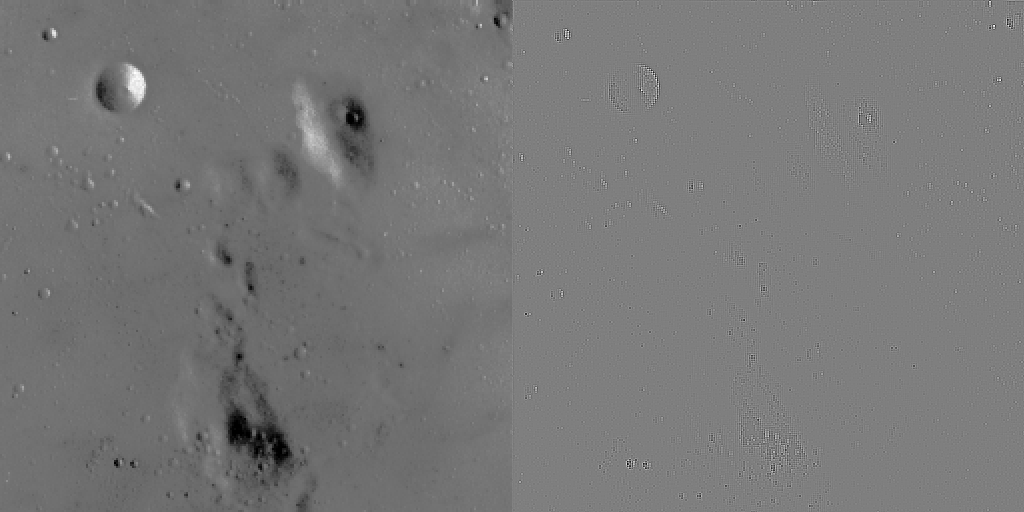
\includegraphics[width=1.00\textwidth]{figures/image_processed/moon_sharpened.png}
    \caption{The original and the sharpened image}
    \label{fig:moon_sharpened}
\end{figure}
\section{Results and Figures}\label{sec:figures}
Answer all the parts of the exercise in an organized and clear manner. You should of course try to get good results in all the exercises, but if you have made a good effort without achieving great performance, a good discussion of possible reasons is just as good. Present your thinking and efforts and discuss possible reasons for good or bad results.

Include plots and/or tables of all relevant results, but make sure you don't overwhelm the reader with too many plots. Have a clear plan about what you want to communicate with a specific plot/figure, and use appropriate labels and comments. Keep in mind that the plots should be as ``readable'' as possible; that is, they should not be too hard to interpret and be reasonably self contained.

There are some important things to consider when exporting figures from MATLAB, most importantly which format you use. Never ever use JPEG for anything that is not a photography or similar. Any figure, like a plot or block diagram, must never be stored as a JPEG\@. If you zoom in on \Cref{fig:constraint_jpg} you can see a lot of noise close to any of the dark curves and lines, this is due to the compression in JPEG\@. \Cref{fig:constraint_jpg} will look horrible both on a screen and on paper.

The PNG format is slightly better for plots, but since it is a raster format (a grid of pixels), it looks ugly if you zoom in. It also looks ugly if you scale it, both on a screen and on paper. Try to avoid PNG if you can. \Cref{fig:constraint_png,fig:constraint_png_large} are both PNG figures; the latter being a larger figure scaled more than the former. Note both how choppy and ugly the blue curve is, and how the different sizes create inconsistent font sizes.

The simplest way to get a reasonably good looking plot is to save it as EPS in MATLAB\@. Do this by clicking ``File'' in the figure window, and the ``Save As\ldots''; choose ``EPS file (*.eps)'' in the ``Save as type:'' menu.\footnote{pdfLatex does not support EPS directly, but since we have loaded the \emph{epstodf} package, this is not a problem.} \Cref{fig:constraint_eps} shows a plot in EPS format. Since EPS is a vector format, the Figure can be scaled and still look good (but mind the font size!). If you zoom in you can see that the curve and the letters/numbers are smooth. A figure in vector format will usually look good both on a screen and on paper.

Note that the size of the actual figure window in MATLAB determines how large the exported figure is. Hence, if you enlarge the figure window before exporting, you will need to scale the figure by a larger factor in the report. This will lead to a tiny font in the figure. There are many better ways of exporting graphics from MATLAB, but they quickly become fairly involved. The above method of exporting to EPS will in most cases give nice figures.

You can write Latex in your MATLAB figures. The script used to create \Cref{fig:constraint_jpg,fig:constraint_eps} is included in \Cref{sec:plot_constraint_m}. Do not use a screen shot of a scope of figure in MATLAB in your report.

\begin{figure}[htb]
	\centering
		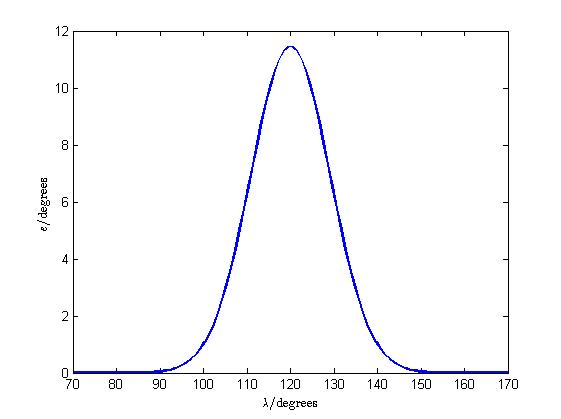
\includegraphics[width=0.8\textwidth]{figures/constraint_jpg.jpg}
	\caption{A plot in JPEG format --- a very bad idea.}
\label{fig:constraint_jpg}
\end{figure}

\begin{figure}[htb]
	\centering
		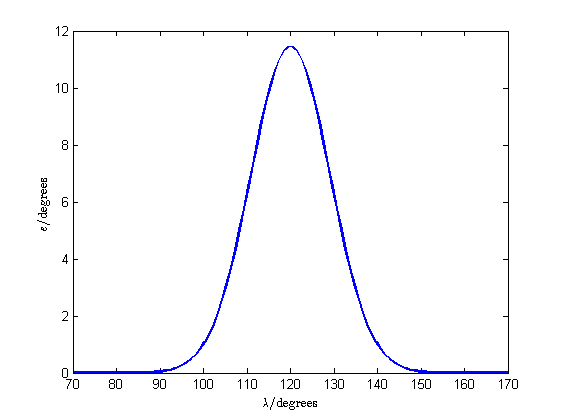
\includegraphics[width=0.8\textwidth]{figures/constraint_png.png}
	\caption{A plot in PNG format --- a bad idea.}
\label{fig:constraint_png}
\end{figure}

\begin{figure}[htb]
	\centering
		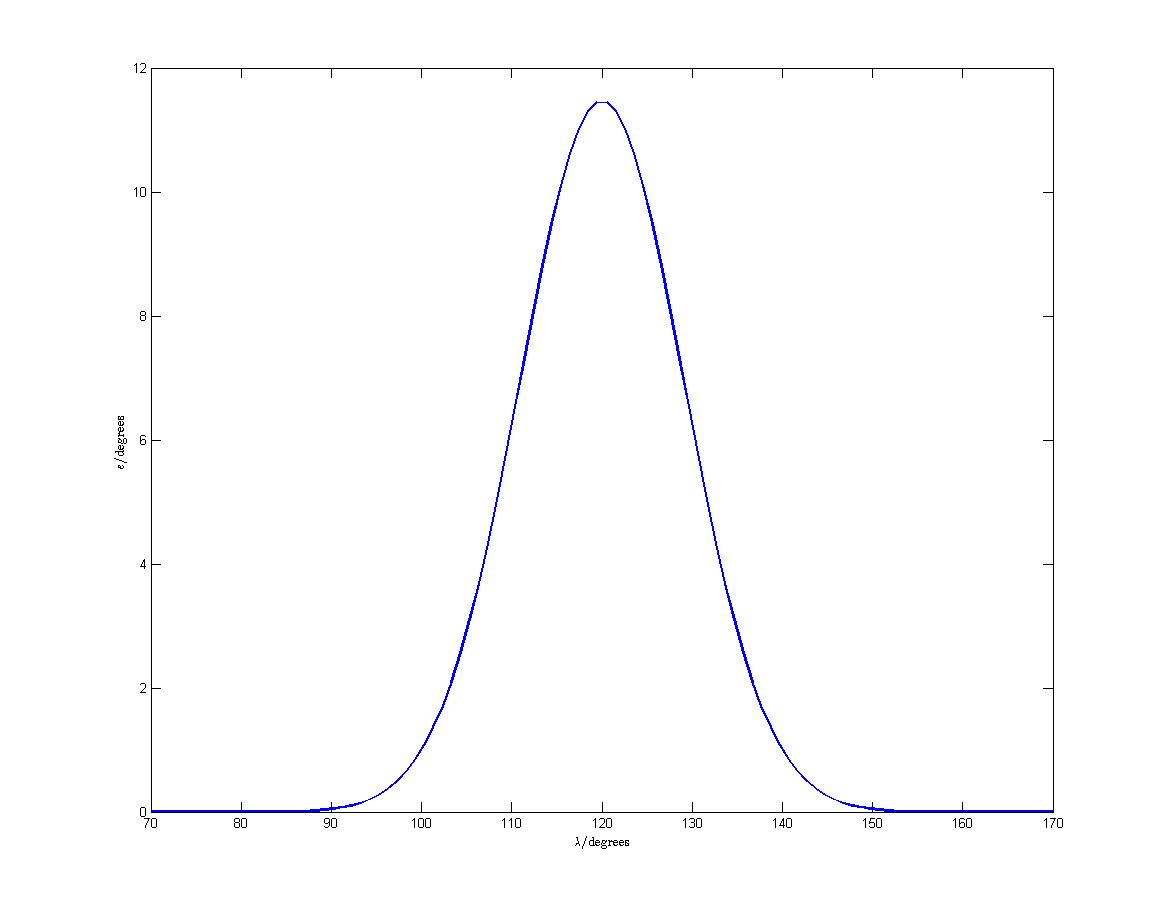
\includegraphics[width=0.8\textwidth]{figures/constraint_png_large.png}
	\caption{A plot in PNG format --- a bad idea. This figure is originally larger than the other PNG figure, but both are scaled to the same size.}
\label{fig:constraint_png_large}
\end{figure}

\begin{figure}[htb]
	\centering
		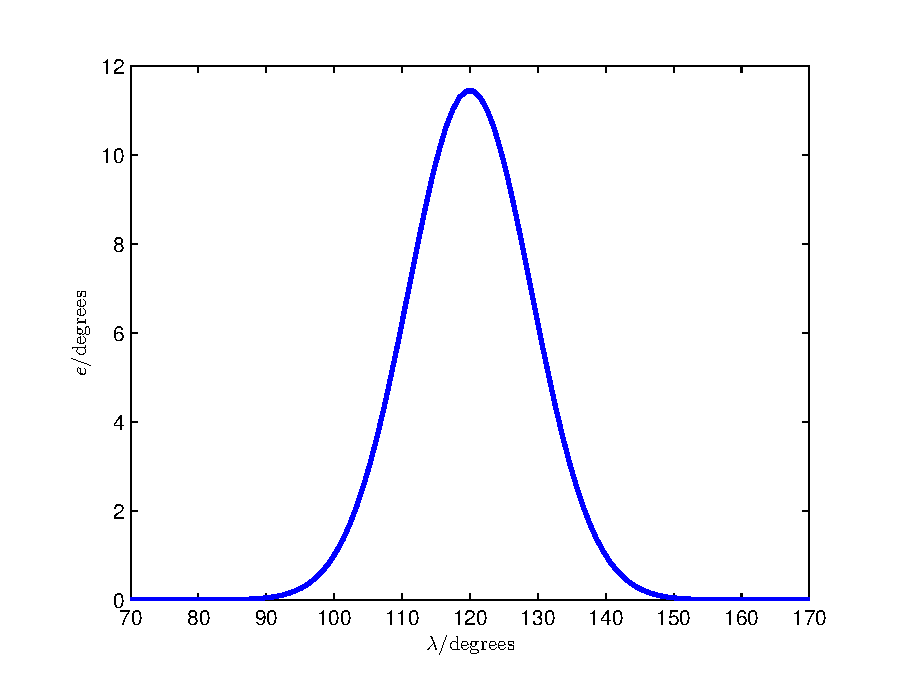
\includegraphics[width=0.8\textwidth]{figures/constraint_eps.eps}
	\caption{A plot in EPS format --- a much better idea.}
\label{fig:constraint_eps}
\end{figure}

Remember to reference all figures in the text. Figures have a number and should be referenced by that number (again, always use dynamic references). They also tend to float around, meaning they generally don't appear where you ask them to in the text. This is fine, do not try to force a figure (or a table) to appear in a particular place. As long a you refer to it, it's easy to find. No figure should be included without being referenced in the text.

If you look at the source code for including figures, you can see that the optional option \verb+[htb]+ has been used. This tells Latex where you wish the figure to appear, in prioritized order. \verb+h+ means ``Here'', t means ``Top of this page'', b means ``Bottom of this page'', and p (not used here) means ``on a Page with only floats (such as figures and tables)''. Note that your wish might not be granted, and this is because Latex actually optimizes the placement of figures. If you start forcing figures to be in specific places, it often leads to really strange layout somewhere else in the document. 

Generally, let Latex handle the documentation layout. This is one of the main reasons to choose Latex over software such as Microsoft Word.

\subsection{Results and Discussion}
All problems should have their own discussion of results. 

Remember: all plots and results need a description, explanation, and discussion.

\section{Task 4: Spinning into gear}
Similarly to Task 3, nothing was required for the report here. 
\section{Task 5: Help! My lighting is wrong!}
\subsection{a)}
See \cref{fig:task5a_light} for the light side of the helicopter and \cref{fig:task5a_dark} for the dark side. 

\begin{figure}[tp]
	\centering
	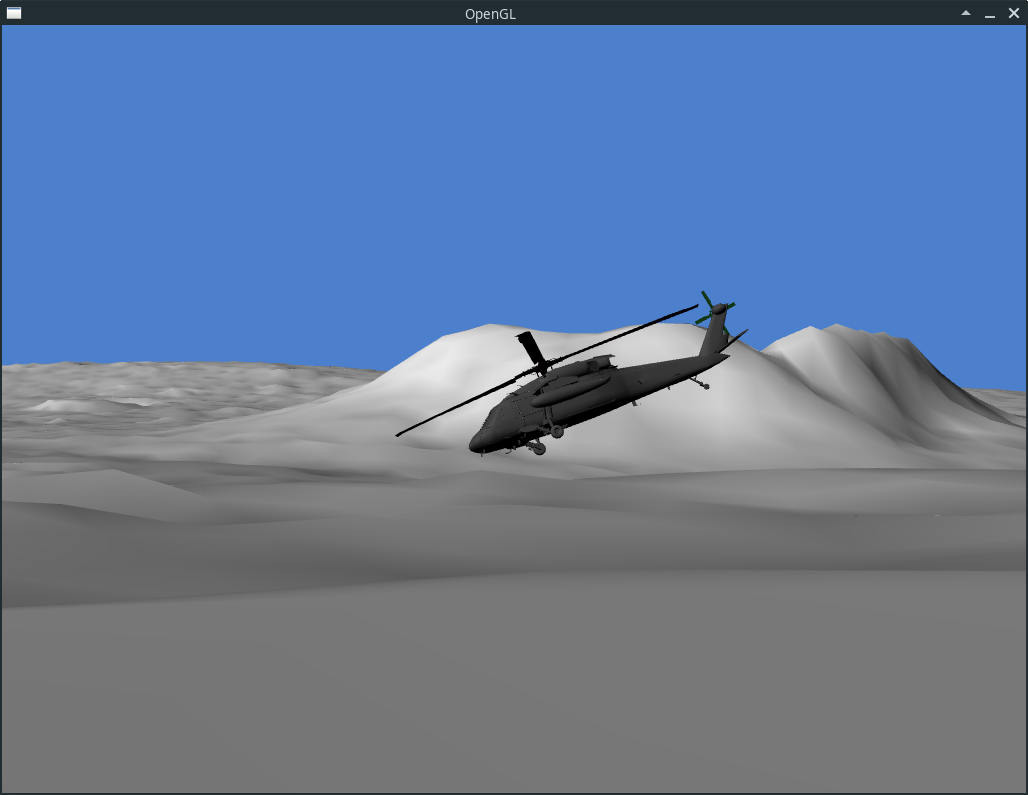
\includegraphics[width=1.00\textwidth]{figures/task5a_light}
	\caption{Light side of the helicopter}
\label{fig:task5a_light}
\end{figure}

\begin{figure}[tp]
	\centering
	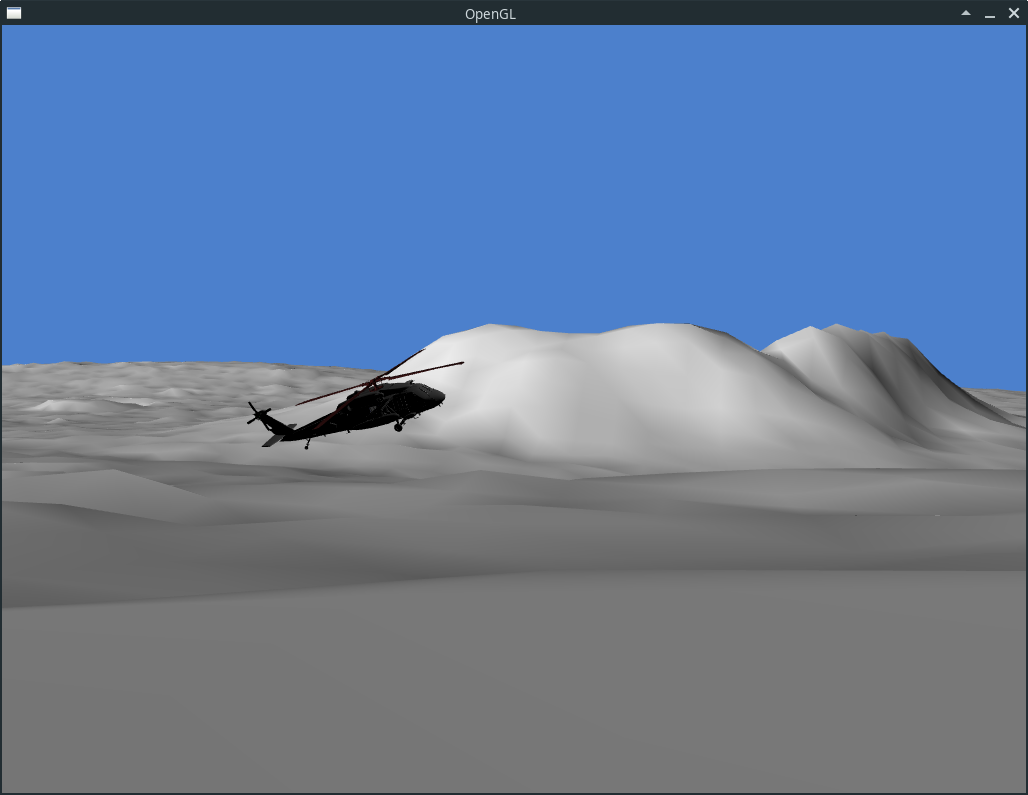
\includegraphics[width=1.00\textwidth]{figures/task5a_dark}
	\caption{Dark side of the helicopter}
\label{fig:task5a_dark}
\end{figure}

\section{Task 6: Time to turn this thing up to 5}
And again, all the code is attached. 
\section{Task 7: Optional Challenges}
\subsection{a)}

\subsection{b)}

\subsection{c)}

\subsection{d)}

\subsection{e)}
See \cref{fig:task7e}
\begin{figure}[tp]
	\centering
	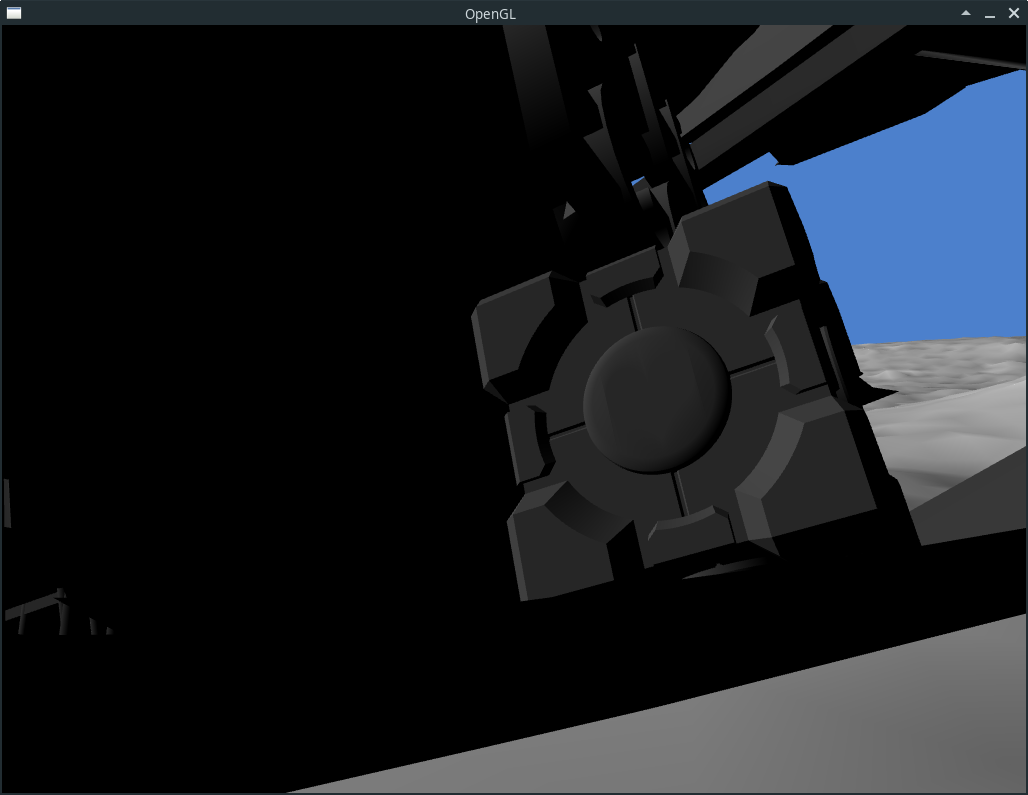
\includegraphics[width=1.00\textwidth]{figures/task7e}
	\caption{Easter egg!}
\label{fig:task7e}
\end{figure}

\subsection{f)}
Extra features (I don't \textit{really} think certain of these deserve extra points, but will list for fun and completeness)

Press SPACE to make the doors open and close again. 

Press C for a \textit{cursed} amount of extra work... Feel free to add any \textit{cursed} music, for atmosphere. My \href{https://www.youtube.com/watch?v=eY52Zsg-KVI}{favourite}.

% \input simply inserts the contents of the file, while \include forces a \newpage.
% See \input vs. \include: http://tex.stackexchange.com/questions/246/when-should-i-use-input-vs-include


% References
\newpage
\addcontentsline{toc}{section}{References}
\printbibliography{}
\label{sec:bibliography}

\end{document}
